\documentclass{article}
\usepackage{clrscode,amsmath,graphicx,grffile}
\title{CLRS 15.3-4}
\author{Peter Danenberg}
\begin{document}
\maketitle

Every station in the factory corresponds to one or more nodes $\{x_0,
  \dots, x_n\}$ in a full binary decision tree $T$; where there are
  $2^{d-1}$ ways to reach every station, and $d$ corresponds to the
  height of $x_i$ in $T$.

See figure \ref{fig:assembly} for a representation of repeating
subproblems.

\begin{figure}[ht]
  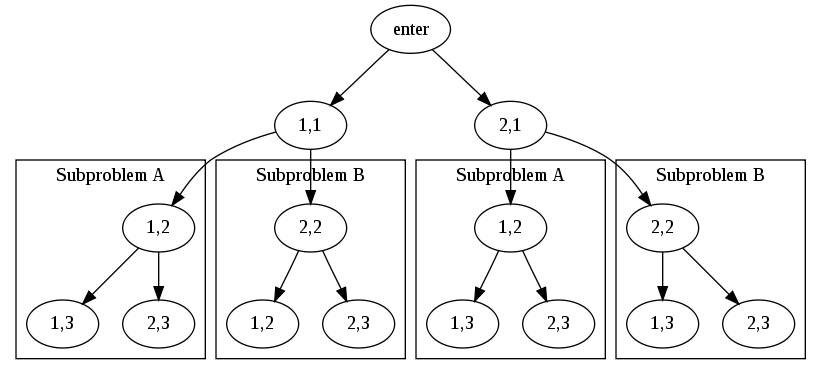
\includegraphics[width=\linewidth]{15.3-4}
  \caption{Assembly line scheduling with overlapping subproblems A and B}
  \label{fig:assembly}
\end{figure}
\end{document}
